\documentclass[12pt,a4paper]{article}
\title{APG4001S Determination of RMS between Precise and Broadcast Ephemerides for Satellite 12}
\date{10 August 2015}
\author{Tim Marsh}

\usepackage{amsmath}
\usepackage{graphicx}
\usepackage{float}
\usepackage{textcomp}
\usepackage{siunitx}
\usepackage{wrapfig}
\usepackage{caption}
\usepackage{subcaption}
\usepackage{pdfpages}
\usepackage{listings}


\graphicspath{ {images/} }
\begin{document}
	
	\pagenumbering{gobble}
	\maketitle
	\begin{figure}[H]
		\centering
		
\includegraphics[width=0.7\linewidth]{UCTcircular_logo1_CMYK}
		\label{fig:UCTcircular_logo1_CMYK}
	\end{figure}
	\newpage
	\pagenumbering{arabic}
	\tableofcontents
%	\listoffigures
	
	\newpage
	\section{Introduction}
		\subsection{Subject of Report}
		The subject if this report is to predict the ephemeris of a single GPS for one orbit. And to then compare our predicted ephemeris to the sp3 file with the correct precise one.
		
		\subsection{Background}
		Every satellite revives a navigation data from ground antenna, that navigation data is then relayed to the users as the navigation message. The navigation message provides all the necessary information to allow the user to perform the positioning service. It includes the Ephemeris parameters, needed to compute the satellite coordinates with enough accuracy, the Time parameters and Clock Corrections, to compute satellite clock offsets and time conversions, the Service Parameters with satellite health information.
		
		This data is all used to refine the reviver coordinates for a specific time(in the case of refining coordinates immediately). The orbit can then be predicted using this information.
		
		Once the orbits have been computed. they can be tested against and preexisting orbit prediction that is kept in the sp3 file.
	
		
		\subsection{Objectives}
		\begin{itemize}
			\item Read the Navigation message file brdc2000.15n
			\item compute the predicted ephemeris
			\item compare the computed predicted ephemiris to the precise ephemiris in the sp3 file igs18540.sp3
			\item display the difference over the course of the orbit
		\end{itemize}
		
		\subsection{Scope and Limitations}
		The program will be written in Python 3. all satellite data must come from the navigation message only and the sp3 file is only for comparing after the computation has happened.
		
	\newpage
	\section{Method}
		\subsection{Algorithm}
			Broadcast ephemeris is attached as Appendix A
		\subsection{Python 3 Program}
			Attached as appendix B
	
	\newpage
	\section{Results}
	The results of the program are as follows:
	
	(with meters difference on the Y-axis and time on the X-axis)
	
	\begin{figure}[H]
	\centering
	\includegraphics[width=0.6\linewidth]{"images/12 - 00"}
	\caption{Sat 12, Epoch 00-00-00}

	\label{fig:12-00}
	\end{figure}
	\begin{figure}[H]
	\centering
	\includegraphics[width=0.6\linewidth]{"images/12 - 04"}
	\caption{Sat 12, Epoch 04-00-00}
	\label{fig:12-04}
	\end{figure}
	\begin{figure}[H]
	\centering
	\includegraphics[width=0.6\linewidth]{"images/12 - 06"}
	\caption{Sat 12, Epoch 06-00-00}
	\label{fig:12-06}
	\end{figure}
	\begin{figure}[H]
	\centering
	\includegraphics[width=0.6\linewidth]{"images/12 - 08"}
	\caption{Sat 12, Epoch 08-00-00}
	\label{fig:12-08}
	\end{figure}
	\begin{figure}[H]
	\centering
	\includegraphics[width=0.6\linewidth]{"images/12 - 10"}
	\caption{Sat 12, Epoch 10-00-00}
	\label{fig:12-10}
	\end{figure}
	\begin{figure}[H]
	\centering
	\includegraphics[width=0.6\linewidth]{"images/12 - 12"}
	\caption{Sat 12, Epoch 12-00-00}
	\label{fig:12-12}
	\end{figure}
	\begin{figure}[H]
	\centering
	\includegraphics[width=0.6\linewidth]{"images/12 - 14"}
	\caption{Sat 12, Epoch 14-00-00}
	\label{fig:12-14}
	\end{figure}
	\begin{figure}[H]
	\centering
	\includegraphics[width=0.6\linewidth]{"images/12 - 16"}
	\caption{Sat 12, Epoch 16-00-00}
	\label{fig:12-16}
	\end{figure}
	\begin{figure}[H]
	\centering
	\includegraphics[width=0.6\linewidth]{"images/12 - 18"}
	\caption{Sat 12, Epoch 18-00-00}
	\label{fig:12-18}
	\end{figure}
	\begin{figure}[H]
	\centering
	\includegraphics[width=0.6\linewidth]{"images/12 - 19"}
	\caption{Sat 12, Epoch 19-59-44}
	\label{fig:12-19}
	\end{figure}

	The Epoch show in the description of the images is the time that the prediction as started
	
	\newpage
	\appendix
	\section{Appendix A}
	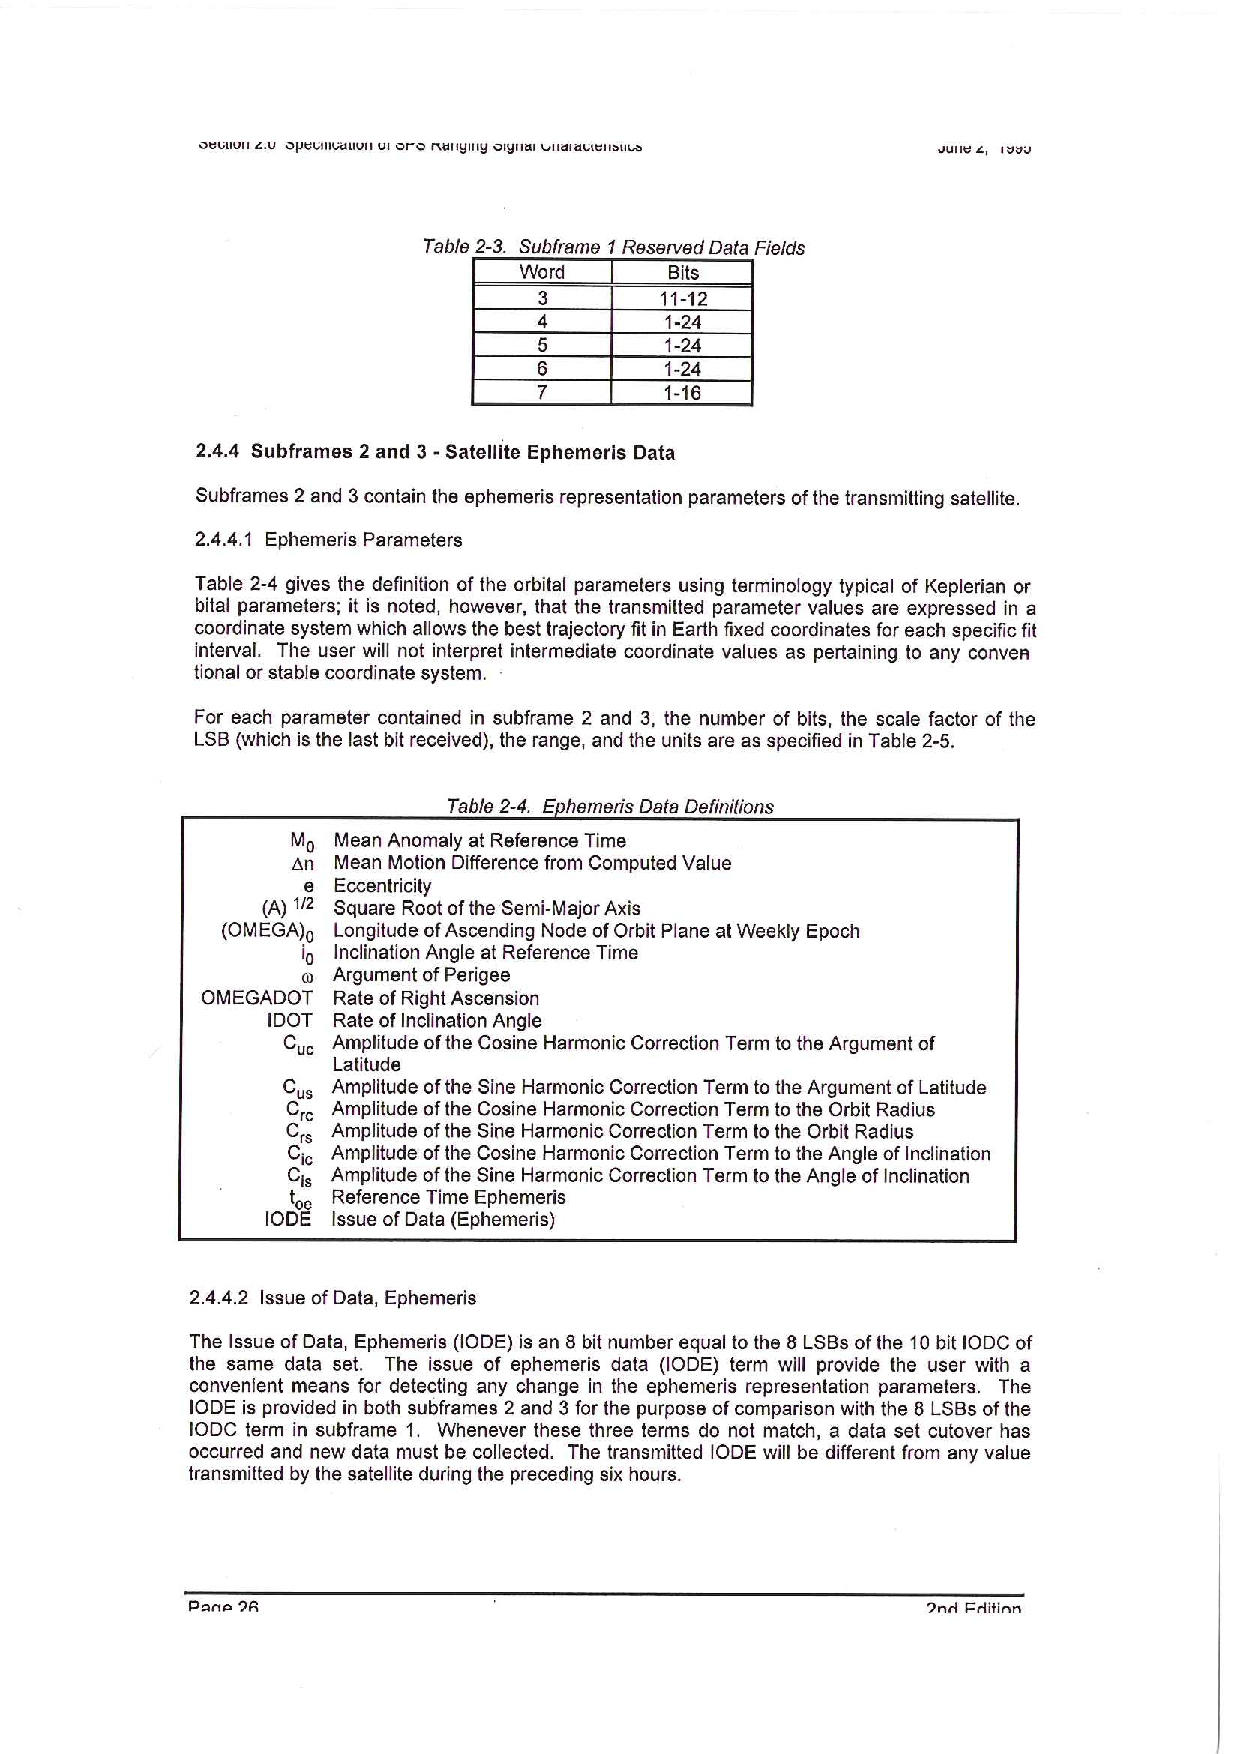
\includepdf[pages=-]{PDF's/algo.pdf}
	\section{Appendix B}
	\lstinputlisting[language=Python]{../main.py}
		
\end{document}	